\chapter{Evaluation}
\label{chap:evaluation}

Dieses Kapitel präsentiert die systematische Evaluation des entwickelten Prototyps. Die Bewertung erfolgt anhand definierter Metriken und validiert die in Kapitel~\ref{chap:anforderungen} spezifizierten funktionalen und nicht-funktionalen Anforderungen. Die Evaluation gliedert sich in die Beschreibung der Testmethodik, die detaillierte Analyse der Einzelkomponenten sowie die Validierung mit realen Siemens-Daten.

\section{Testmethodik}
\label{sec:testmethodik}

Die Evaluation des Systems erfordert eine sorgfältige Definition der Testbedingungen, um reproduzierbare und aussagekräftige Ergebnisse zu gewährleisten. Dieser Abschnitt beschreibt den verwendeten Testdatensatz, die angewandten Evaluationsmetriken sowie die Testumgebung.

\subsection{Testdatensatz und Ground Truth}
\label{subsec:testdatensatz}

Zur Evaluation des Systems wurde ein dedizierter Testdatensatz erstellt, der von den Trainingsdaten strikt getrennt ist. Diese Trennung ist essenziell, um eine unvoreingenommene Bewertung der Generalisierungsfähigkeit des Modells zu gewährleisten.

\subsubsection{Datensatzzusammensetzung}

Der Testdatensatz umfasst Gleispläne unterschiedlicher Komplexität und Qualitätsstufen, um die Robustheit des Systems unter variierenden Bedingungen zu prüfen. Tabelle~\ref{tab:testdatensatz_statistik} zeigt die statistischen Kennzahlen des Testdatensatzes.

\begin{table}[H]
\centering
\begin{tabular}{|l|r|}
\hline
\textbf{Attribut} & \textbf{Wert} \\
\hline
Anzahl Testpläne & X \\
Gesamtzahl Seiten & X \\
Annotierte Symbole (gesamt) & X \\
\hspace{3mm} davon Signale & X \\
\hspace{3mm} davon Koordinaten & X \\
\hspace{3mm} davon GKS-Platten & X \\
\hspace{3mm} davon Weichenblöcke & X \\
\hspace{3mm} davon sonstige Klassen & X \\
Annotierte Textfelder & X \\
Plantypen & A-Typ Gleispläne \\
Auflösungsbereich & 300--500 DPI \\
\hline
\end{tabular}
\caption{Statistiken des Testdatensatzes}
\label{tab:testdatensatz_statistik}
\end{table}

\subsubsection{Ground-Truth-Erstellung}

Die Ground-Truth-Annotationen wurden manuell durch den Autor unter Verwendung des Annotationstools CVAT erstellt. Für jedes Symbol im Testdatensatz wurden folgende Informationen erfasst:

\begin{itemize}
    \item \textbf{Objektklasse}: Zuordnung zu einer der 13 definierten Symbolklassen
    \item \textbf{Oriented Bounding Box}: Präzise Umrandung durch $(c_x, c_y, w, h, \theta)$
    \item \textbf{Textinhalt}: Der korrekte OCR-Text für Symbole mit Beschriftung
    \item \textbf{Verknüpfungen}: Die korrekten Symbol-Text-Assoziationen
\end{itemize}

Die Annotationsrichtlinien wurden konsistent mit den Trainingsannotationen gehalten, um eine valide Vergleichsbasis zu schaffen. Zur Qualitätssicherung wurden X\% der Annotationen durch einen zweiten Prüfer verifiziert.

\subsubsection{Qualitätskategorien}

Um die Robustheit des Systems unter verschiedenen Bedingungen zu evaluieren, wurden die Testpläne in drei Qualitätskategorien eingeteilt:

\begin{table}[H]
\centering
\begin{tabular}{|l|p{8cm}|r|}
\hline
\textbf{Kategorie} & \textbf{Charakteristik} & \textbf{Anzahl} \\
\hline
Gut & Hohe Auflösung, klare Linien, keine Artefakte & X \\
Mittel & Moderate Auflösung, leichte Artefakte oder Rauschen & X \\
Schwierig & Niedrige Auflösung, starke Artefakte, Scan-Probleme & X \\
\hline
\end{tabular}
\caption{Qualitätskategorien der Testpläne}
\label{tab:qualitaetskategorien}
\end{table}

\subsection{Evaluationsmetriken}
\label{subsec:evaluationsmetriken}

Die Bewertung des Systems erfolgt auf mehreren Ebenen mit jeweils spezifischen Metriken. Die nachfolgend definierten Metriken ermöglichen eine differenzierte Analyse der einzelnen Pipeline-Komponenten sowie der Gesamtsystemleistung.

\subsubsection{Metriken für die Objekterkennung}

Für die Bewertung der YOLO-basierten Objekterkennung werden die folgenden Standardmetriken verwendet:

\textbf{Precision} quantifiziert den Anteil korrekter Detektionen an allen vom Modell vorhergesagten Detektionen:
\begin{equation}
\text{Precision} = \frac{TP}{TP + FP}
\end{equation}

\textbf{Recall} misst den Anteil der erkannten Objekte an allen tatsächlich vorhandenen Objekten:
\begin{equation}
\text{Recall} = \frac{TP}{TP + FN}
\end{equation}

\textbf{F1-Score} bildet das harmonische Mittel aus Precision und Recall:
\begin{equation}
F_1 = 2 \cdot \frac{\text{Precision} \cdot \text{Recall}}{\text{Precision} + \text{Recall}}
\end{equation}

\textbf{Mean Average Precision (mAP)} aggregiert die Precision über verschiedene Recall-Stufen und IoU-Schwellenwerte. Es werden zwei Varianten berichtet:
\begin{itemize}
    \item \textbf{mAP@0.5}: Durchschnittliche Precision bei einer IoU-Schwelle von 50\%
    \item \textbf{mAP@0.5:0.95}: Durchschnitt über IoU-Schwellen von 50\% bis 95\% in 5\%-Schritten
\end{itemize}

Die \textbf{Intersection over Union (IoU)} definiert den Überlappungsgrad zwischen vorhergesagter Box $B_p$ und Ground-Truth-Box $B_{gt}$:
\begin{equation}
\text{IoU}(B_p, B_{gt}) = \frac{|B_p \cap B_{gt}|}{|B_p \cup B_{gt}|}
\end{equation}

Eine Detektion gilt als True Positive, wenn $\text{IoU} \geq \tau_{IoU}$ mit der zugeordneten Ground-Truth-Box.

\subsubsection{Metriken für die Texterkennung}

Die OCR-Leistung wird durch folgende Metriken quantifiziert:

\textbf{Character Error Rate (CER)} misst die Zeichenfehlerrate basierend auf der Levenshtein-Distanz:
\begin{equation}
\text{CER} = \frac{S + D + I}{N}
\end{equation}
wobei $S$ die Anzahl der Substitutionen, $D$ die Anzahl der Deletionen, $I$ die Anzahl der Insertionen und $N$ die Gesamtanzahl der Zeichen im Ground-Truth-Text bezeichnet.

\textbf{Field Accuracy Rate (FAR)} gibt den Anteil der vollständig korrekt erkannten Textfelder an:
\begin{equation}
\text{FAR} = \frac{\text{Anzahl exakt übereinstimmender Felder}}{\text{Gesamtanzahl Felder}}
\end{equation}

\textbf{Regex-Validierungsrate} misst den Anteil der OCR-Ergebnisse, die das klassenspezifische Formatmuster erfüllen:
\begin{equation}
\text{Regex-Rate} = \frac{\text{Anzahl regex-valider Ergebnisse}}{\text{Gesamtanzahl OCR-Ergebnisse}}
\end{equation}

\subsubsection{Metriken für die Symbol-Text-Verknüpfung}

Die Linking-Qualität wird durch folgende Metriken bewertet:

\textbf{Linking Accuracy} misst den Anteil korrekter Verknüpfungen:
\begin{equation}
\text{Linking Accuracy} = \frac{\text{Korrekte Verknüpfungen}}{\text{Gesamtanzahl Verknüpfungen}}
\end{equation}

\textbf{False Positive Linking Rate} erfasst fälschlicherweise hergestellte Verknüpfungen:
\begin{equation}
\text{FP-Linking} = \frac{\text{Falsche Verknüpfungen}}{\text{Gesamtanzahl vom System erstellter Verknüpfungen}}
\end{equation}

\textbf{Missing Link Rate} quantifiziert fehlende Verknüpfungen:
\begin{equation}
\text{Missing Links} = \frac{\text{Fehlende Verknüpfungen}}{\text{Gesamtanzahl erwarteter Verknüpfungen}}
\end{equation}

\subsubsection{End-to-End Systemmetrik}

Die Gesamtsystemleistung wird durch die \textbf{End-to-End Accuracy} gemessen, die dem in Anforderung NFA-003 definierten Zielwert entspricht:
\begin{equation}
\text{E2E Accuracy} = \frac{\text{Vollständig korrekt extrahierte Objekte}}{\text{Gesamtanzahl Objekte}}
\end{equation}

Ein Objekt gilt als \enquote{vollständig korrekt extrahiert}, wenn alle folgenden Bedingungen erfüllt sind:
\begin{enumerate}
    \item Das Symbol wurde korrekt detektiert (IoU $\geq$ 0.5 mit Ground Truth)
    \item Die Klassifikation ist korrekt
    \item Der OCR-Text stimmt exakt mit dem Ground Truth überein
    \item Alle erforderlichen Verknüpfungen (z.B. zu Koordinaten) sind korrekt
\end{enumerate}

\subsection{Testumgebung}
\label{subsec:testumgebung}

Die Evaluation wurde auf einer standardisierten Hardware- und Softwarekonfiguration durchgeführt, um reproduzierbare Ergebnisse zu gewährleisten. Tabelle~\ref{tab:testumgebung} fasst die technischen Spezifikationen zusammen.

\begin{table}[H]
\centering
\begin{tabular}{|l|l|}
\hline
\textbf{Komponente} & \textbf{Spezifikation} \\
\hline
\multicolumn{2}{|c|}{\textit{Hardware (Inferenz)}} \\
\hline
CPU & Intel Core i7-10700 (8 Kerne, 2.9 GHz) \\
RAM & 32 GB DDR4 \\
GPU & Keine (CPU-only Inferenz) \\
Speicher & 512 GB SSD \\
\hline
\multicolumn{2}{|c|}{\textit{Hardware (Training)}} \\
\hline
GPU & NVIDIA T4 (AWS g4dn.xlarge) \\
VRAM & 16 GB \\
\hline
\multicolumn{2}{|c|}{\textit{Software}} \\
\hline
Betriebssystem & Windows 10 / Ubuntu 22.04 \\
Python & 3.9.16 \\
PyTorch & 2.0.1 \\
Ultralytics & 8.0.196 \\
PaddleOCR & 2.7.0 \\
Tesseract & 5.3.0 \\
\hline
\end{tabular}
\caption{Hardware- und Softwarekonfiguration der Testumgebung}
\label{tab:testumgebung}
\end{table}

Die Wahl einer CPU-basierten Inferenzumgebung reflektiert die Anforderung NFA-001, die eine On-Premise-Verarbeitung auf Standard-Workstations ohne dedizierte GPU vorsieht. Alle Zeitmessungen wurden als Mittelwert über drei Durchläufe berechnet, um Varianz durch Systemlast zu minimieren.

\section{Ergebnisanalyse}
\label{sec:ergebnisanalyse}

Dieser Abschnitt präsentiert die quantitativen Evaluationsergebnisse der einzelnen Pipeline-Komponenten sowie des Gesamtsystems. Die Ergebnisse werden im Kontext der definierten Anforderungen interpretiert.

\subsection{Objekterkennungsleistung}
\label{subsec:detection_eval}

Die Objekterkennung bildet die fundamentale Stufe der Extraktionspipeline. Die Qualität der YOLO-Detektionen determiniert maßgeblich die erreichbare Gesamtgenauigkeit des Systems.

\subsubsection{Gesamtleistung auf dem Testdatensatz}

Das trainierte YOLOv8l-OBB Modell wurde auf dem vollständigen Testdatensatz evaluiert. Tabelle~\ref{tab:detection_overall} zeigt die aggregierten Metriken über alle Symbolklassen.

\begin{table}[H]
\centering
\begin{tabular}{|l|r|}
\hline
\textbf{Metrik} & \textbf{Wert} \\
\hline
Precision (Durchschnitt) & X.XX\% \\
Recall (Durchschnitt) & X.XX\% \\
F1-Score & X.XX\% \\
mAP@0.5 & X.XX\% \\
mAP@0.5:0.95 & X.XX\% \\
\hline
\end{tabular}
\caption{Aggregierte Detektionsmetriken auf dem Testdatensatz}
\label{tab:detection_overall}
\end{table}

Der erreichte Recall von X.XX\% erfüllt die Anforderung FA-001, die eine Mindesterkennungsrate von 90\% fordert. Die hohe Precision von X.XX\% zeigt, dass das Modell nur wenige Falschdetektionen produziert.

\subsubsection{Klassenspezifische Analyse}

Die Detektionsleistung variiert erwartungsgemäß zwischen den verschiedenen Symbolklassen. Tabelle~\ref{tab:detection_per_class} zeigt die klassenspezifischen Metriken.

\begin{table}[H]
\centering
\small
\begin{tabular}{|l|r|r|r|r|r|}
\hline
\textbf{Klasse} & \textbf{Instanzen} & \textbf{Precision} & \textbf{Recall} & \textbf{mAP@0.5} & \textbf{mAP@0.5:0.95} \\
\hline
signal & X & X.XX & X.XX & X.XX & X.XX \\
coordinate & X & X.XX & X.XX & X.XX & X.XX \\
gks\_festkodiert & X & X.XX & X.XX & X.XX & X.XX \\
gks\_gesteuert & X & X.XX & X.XX & X.XX & X.XX \\
weichen\_block & X & X.XX & X.XX & X.XX & X.XX \\
haltepunkt & X & X.XX & X.XX & X.XX & X.XX \\
isolierstoß & X & X.XX & X.XX & X.XX & X.XX \\
sverbinder & X & X.XX & X.XX & X.XX & X.XX \\
gm\_block & X & X.XX & X.XX & X.XX & X.XX \\
prellblock & X & X.XX & X.XX & X.XX & X.XX \\
haltetafel & X & X.XX & X.XX & X.XX & X.XX \\
endeweichen & X & X.XX & X.XX & X.XX & X.XX \\
weichengruppeende & X & X.XX & X.XX & X.XX & X.XX \\
\hline
\textbf{Durchschnitt} & \textbf{X} & \textbf{X.XX} & \textbf{X.XX} & \textbf{X.XX} & \textbf{X.XX} \\
\hline
\end{tabular}
\caption{Klassenspezifische Detektionsmetriken auf dem Testdatensatz}
\label{tab:detection_per_class}
\end{table}

Die Analyse der klassenspezifischen Ergebnisse offenbart mehrere Beobachtungen:

\begin{itemize}
    \item \textbf{Beste Performance}: Die Klassen \textit{signal} und \textit{coordinate} zeigen die höchsten Erkennungsraten, was auf ihre hohe Häufigkeit im Trainingsdatensatz und ihre distinktive visuelle Erscheinung zurückzuführen ist.
    
    \item \textbf{Herausforderungen bei seltenen Klassen}: Klassen mit wenigen Trainingsbeispielen wie \textit{endeweichen} und \textit{haltetafel} zeigen erwartungsgemäß niedrigere Recall-Werte, da das Modell weniger Gelegenheit hatte, deren Varianz zu lernen.
    
    \item \textbf{Konfusion ähnlicher Klassen}: Die Klassen \textit{gks\_festkodiert} und \textit{gks\_gesteuert} weisen aufgrund ihrer hohen visuellen Ähnlichkeit gelegentliche Verwechslungen auf.
\end{itemize}

\subsubsection{Rotationsinvarianz}

Zur Validierung der Anforderung FA-002 (Rotationsinvarianz) wurde die Detektionsleistung in Abhängigkeit vom Rotationswinkel der Symbole analysiert. Die Ground-Truth-Annotationen enthalten den Rotationswinkel $\theta$ für jedes Symbol, der in Winkelbereiche diskretisiert wurde.

\begin{table}[H]
\centering
\begin{tabular}{|l|r|r|r|r|}
\hline
\textbf{Winkelbereich} & \textbf{Instanzen} & \textbf{Recall} & \textbf{Precision} & \textbf{Winkelfehler (Ø)} \\
\hline
$0^\circ \pm 15^\circ$ (horizontal) & X & X.XX\% & X.XX\% & X.X° \\
$90^\circ \pm 15^\circ$ (vertikal) & X & X.XX\% & X.XX\% & X.X° \\
$45^\circ \pm 15^\circ$ (diagonal) & X & X.XX\% & X.XX\% & X.X° \\
$135^\circ \pm 15^\circ$ (diagonal) & X & X.XX\% & X.XX\% & X.X° \\
Sonstige Winkel & X & X.XX\% & X.XX\% & X.X° \\
\hline
\end{tabular}
\caption{Detektionsleistung nach Rotationswinkel}
\label{tab:detection_rotation}
\end{table}

Die Ergebnisse belegen, dass das YOLOv8-OBB Modell eine robuste Detektion über alle Orientierungen hinweg erreicht. Der durchschnittliche Winkelfehler von X.X° zeigt, dass die OBB-Regression die Symbolorientierung präzise erfasst, was für die nachfolgende OCR-Verarbeitung essenziell ist.

\subsubsection{Fehleranalyse}

Zur systematischen Identifikation von Schwachstellen wurden die Detektionsfehler kategorisiert. Abbildung~\ref{fig:detection_error_analysis} visualisiert die Verteilung der Fehlertypen.

\begin{figure}[H]
\centering
\begin{tikzpicture}
% Die Summe der Zahlen sollte idealerweise 100 ergeben (bei Prozent)
% oder die Summe deiner Fehlerfälle sein.
\pie[
    text=legend,      % Legende statt Text im Diagramm
    radius=3,
    color={red!60, orange!60, yellow!60, green!60, blue!60},
    sum=auto          % Berechnet die Prozentanteile automatisch
]{
    35/Übersehen (kleine Symbole),
    25/Falsche Klasse,
    20/Duplikate an Tile-Grenzen,
    15/Hintergrund-Verwechslung,
    5/Sonstige
}
\end{tikzpicture}
\caption{Verteilung der Detektionsfehler nach Kategorie}
\label{fig:detection_error_analysis}
\end{figure}

Die häufigsten Fehlerursachen sind:

\begin{enumerate}
    \item \textbf{Übersehene kleine Symbole (X\%)}: Besonders bei niedriger Auflösung oder starker Verkleinerung werden kleine Symbole wie Isolierstöße gelegentlich nicht erkannt.
    
    \item \textbf{Klassifikationsfehler (X\%)}: Visuell ähnliche Symboltypen werden verwechselt, insbesondere innerhalb der GKS-Familie.
    
    \item \textbf{Tile-Grenz-Artefakte (X\%)}: Trotz der implementierten Überlappung und NMS treten vereinzelt Duplikate oder geteilte Detektionen an Kachelgrenzen auf.
\end{enumerate}

\subsection{OCR-Leistungsanalyse}
\label{subsec:ocr_eval}

Die OCR-Komponente extrahiert die textuellen Informationen aus den detektierten Symbolbereichen. Die Evaluation erfolgt auf allen Textfeldern des Testdatensatzes mit bekanntem Ground-Truth-Text.

\subsubsection{Gesamtleistung der OCR-Pipeline}

Tabelle~\ref{tab:ocr_overall} zeigt die aggregierten OCR-Metriken über alle Texttypen.

\begin{table}[H]
\centering
\begin{tabular}{|l|r|}
\hline
\textbf{Metrik} & \textbf{Wert} \\
\hline
Character Error Rate (CER) & X.XX\% \\
Field Accuracy Rate (exakte Übereinstimmung) & X.XX\% \\
Regex-Validierungsrate & X.XX\% \\
\hline
\end{tabular}
\caption{Aggregierte OCR-Metriken auf dem Testdatensatz}
\label{tab:ocr_overall}
\end{table}

Die erreichte CER von X.XX\% und die Field Accuracy von X.XX\% demonstrieren die Effektivität der Multi-Engine-OCR-Pipeline. Die hohe Regex-Validierungsrate zeigt, dass die extrahierten Texte in der überwiegenden Mehrheit dem erwarteten Format entsprechen.

\subsubsection{Klassenspezifische OCR-Leistung}

Die OCR-Anforderungen variieren je nach Symbolklasse. Tabelle~\ref{tab:ocr_per_class} differenziert die Leistung nach Texttyp.

\begin{table}[H]
\centering
\begin{tabular}{|l|r|r|r|r|}
\hline
\textbf{Texttyp} & \textbf{Anzahl} & \textbf{CER} & \textbf{Field Accuracy} & \textbf{Regex-Rate} \\
\hline
Signalbezeichnung & X & X.XX\% & X.XX\% & X.XX\% \\
Koordinatentext & X & X.XX\% & X.XX\% & X.XX\% \\
GKS-Nummer & X & X.XX\% & X.XX\% & X.XX\% \\
Fahrtrichtung (A/B) & X & X.XX\% & X.XX\% & X.XX\% \\
Sonstige Texte & X & X.XX\% & X.XX\% & X.XX\% \\
\hline
\textbf{Gesamt} & \textbf{X} & \textbf{X.XX\%} & \textbf{X.XX\%} & \textbf{X.XX\%} \\
\hline
\end{tabular}
\caption{Klassenspezifische OCR-Metriken}
\label{tab:ocr_per_class}
\end{table}

\textbf{Beobachtungen:}
\begin{itemize}
    \item \textbf{Signalbezeichnungen} erzielen hohe Genauigkeit aufgrund ihrer standardisierten Formatierung und typischerweise guten Lesbarkeit.
    
    \item \textbf{Koordinatentexte} zeigen gelegentlich Probleme bei der Erkennung von Dezimaltrennzeichen (Punkt vs. Komma) und bei der Unterscheidung von Ziffern in dichter Gruppierung.
    
    \item \textbf{Fahrtrichtungsangaben} (A/B) erreichen nahezu perfekte Genauigkeit, da nur zwei mögliche Werte existieren und diese typischerweise klar lesbar sind.
\end{itemize}

\subsubsection{Engine-Vergleich}

Die Multi-Engine-Architektur nutzt PaddleOCR als Primärengine mit Tesseract als Fallback. Tabelle~\ref{tab:ocr_engine_comparison} vergleicht die Leistung der Engines.

\begin{table}[H]
\centering
\begin{tabular}{|l|r|r|r|r|}
\hline
\textbf{Engine} & \textbf{CER (horiz.)} & \textbf{CER (rotiert)} & \textbf{Ø Inferenzzeit} & \textbf{Nutzungsanteil} \\
\hline
PaddleOCR & X.XX\% & X.XX\% & X ms & X\% \\
Tesseract (Fallback) & X.XX\% & X.XX\% & X ms & X\% \\
\hline
\end{tabular}
\caption{Vergleich der OCR-Engines}
\label{tab:ocr_engine_comparison}
\end{table}

PaddleOCR zeigt konsistent bessere Ergebnisse, insbesondere bei rotierten Texten. Der Tesseract-Fallback wird in X\% der Fälle aktiviert, typischerweise bei niedrigen PaddleOCR-Konfidenzwerten oder bei stark pixeligen Textregionen.

\subsubsection{Effektivität des Dual-Angle-Routing}

Das Dual-Angle-Routing-System verarbeitet jeden Textausschnitt in zwei Orientierungen (Original und 90°-Rotation) und wählt das Ergebnis mit höherer Konfidenz und Regex-Validierung. Tabelle~\ref{tab:dual_angle_effectiveness} quantifiziert den Beitrag dieses Ansatzes.

\begin{table}[H]
\centering
\begin{tabular}{|l|r|}
\hline
\textbf{Metrik} & \textbf{Wert} \\
\hline
Fälle mit Pfad A (Original) gewählt & X\% \\
Fälle mit Pfad B (90°-Rotation) gewählt & X\% \\
Genauigkeitsverbesserung durch Dual-Path (vs. Single-Path) & +X.XX\% \\
Zusätzliche Verarbeitungszeit durch Dual-Path & +X\% \\
\hline
\end{tabular}
\caption{Effektivität des Dual-Angle-Routing-Systems}
\label{tab:dual_angle_effectiveness}
\end{table}

Der Dual-Path-Ansatz verbessert die Gesamtgenauigkeit um X.XX Prozentpunkte bei einem moderaten Zeitoverhead von X\%. Besonders bei Textfeldern ohne eindeutige Orientierungsinformation (z.B. quadratische Bounding Boxes) liefert dieser Mechanismus signifikante Verbesserungen.

\subsubsection{Fehleranalyse}

Die systematische Analyse der OCR-Fehler identifiziert wiederkehrende Muster, die in Tabelle~\ref{tab:ocr_errors} kategorisiert sind.

\begin{table}[H]
\centering
\begin{tabular}{|l|r|l|}
\hline
\textbf{Fehlertyp} & \textbf{Häufigkeit} & \textbf{Beispiel} \\
\hline
O/0 Verwechslung & X\% & \enquote{A1O2} statt \enquote{A102} \\
1/I/l Verwechslung & X\% & \enquote{Al02} statt \enquote{A102} \\
Fehlende Zeichen & X\% & \enquote{A12} statt \enquote{A123} \\
Zusätzliche Zeichen & X\% & \enquote{A1023} statt \enquote{A102} \\
Dezimaltrennzeichen & X\% & \enquote{18,1606} statt \enquote{18.1606} \\
Rauschen/Artefakte & X\% & \enquote{A1\_02} statt \enquote{A102} \\
Sonstige & X\% & --- \\
\hline
\end{tabular}
\caption{Kategorisierung der OCR-Fehler}
\label{tab:ocr_errors}
\end{table}

Die häufigsten Fehler (O/0, 1/I/l) sind klassische OCR-Verwechslungen, die durch die domänenspezifische Validierung (Regex-Patterns) und das Fuzzy-Matching weitgehend korrigiert werden können.

\subsection{Linking-Genauigkeit}
\label{subsec:linking_eval}

Die Symbol-Text-Verknüpfung stellt die semantische Korrektheit der extrahierten Daten sicher. Die Evaluation prüft, ob die richtigen Textfelder den korrekten Symbolen zugeordnet werden.

\subsubsection{Gesamtleistung des Linking-Moduls}

Tabelle~\ref{tab:linking_overall} zeigt die aggregierten Linking-Metriken.

\begin{table}[H]
\centering
\begin{tabular}{|l|r|}
\hline
\textbf{Metrik} & \textbf{Wert} \\
\hline
Linking Accuracy (gesamt) & X.XX\% \\
False Positive Linking Rate & X.XX\% \\
Missing Link Rate & X.XX\% \\
\hline
\end{tabular}
\caption{Aggregierte Linking-Metriken}
\label{tab:linking_overall}
\end{table}

\subsubsection{Verknüpfungstyp-spezifische Analyse}

Die Linking-Anforderungen und -Komplexität variieren je nach Verknüpfungstyp. Tabelle~\ref{tab:linking_per_type} differenziert die Ergebnisse.

\begin{table}[H]
\centering
\begin{tabular}{|l|r|r|r|r|}
\hline
\textbf{Verknüpfungstyp} & \textbf{Anzahl} & \textbf{Korrekt} & \textbf{Falsch} & \textbf{Fehlend} \\
\hline
Signal $\rightarrow$ Koordinate & X & X.XX\% & X.XX\% & X.XX\% \\
Signal $\rightarrow$ Signalbezeichnung & X & X.XX\% & X.XX\% & X.XX\% \\
GKS $\rightarrow$ Koordinate & X & X.XX\% & X.XX\% & X.XX\% \\
GKS $\rightarrow$ GKS-Nummer & X & X.XX\% & X.XX\% & X.XX\% \\
Weiche $\rightarrow$ Koordinate(n) & X & X.XX\% & X.XX\% & X.XX\% \\
Haltepunkt-Gruppierung & X & X.XX\% & X.XX\% & X.XX\% \\
\hline
\textbf{Gesamt} & \textbf{X} & \textbf{X.XX\%} & \textbf{X.XX\%} & \textbf{X.XX\%} \\
\hline
\end{tabular}
\caption{Linking-Genauigkeit nach Verknüpfungstyp}
\label{tab:linking_per_type}
\end{table}

\subsubsection{Fahrtrichtungsdetektion}

Die geometrische Ableitung der Fahrtrichtung (FA-006) aus der Signal-Balise-Relation wird separat evaluiert.

\begin{table}[H]
\centering
\begin{tabular}{|l|r|r|r|}
\hline
\textbf{Ground Truth} & \textbf{Erkannt als A} & \textbf{Erkannt als B} & \textbf{Nicht erkannt} \\
\hline
Fahrtrichtung A & X & X & X \\
Fahrtrichtung B & X & X & X \\
\hline
\end{tabular}
\caption{Konfusionsmatrix der Fahrtrichtungsdetektion}
\label{tab:direction_confusion}
\end{table}

Die Gesamtgenauigkeit der Fahrtrichtungsdetektion beträgt X.XX\%. Fehler treten primär auf, wenn die zugehörige Balise nicht detektiert wurde oder die geometrische Relation ambig ist.

\subsubsection{Beitrag des Adaptive Learning}

Der adaptive Lernmechanismus (vgl. Abschnitt~\ref{sec:Koordinatentransformation}) verbessert die Linking-Genauigkeit durch Mustererkennung aus erfolgreichen Verknüpfungen. Tabelle~\ref{tab:adaptive_learning_impact} quantifiziert den Effekt.

\begin{table}[H]
\centering
\begin{tabular}{|l|r|r|}
\hline
\textbf{Konfiguration} & \textbf{Linking Accuracy} & \textbf{Missing Links} \\
\hline
Ohne Adaptive Learning & X.XX\% & X.XX\% \\
Mit Adaptive Learning & X.XX\% & X.XX\% \\
\hline
\textbf{Verbesserung} & \textbf{+X.XX\%} & \textbf{-X.XX\%} \\
\hline
\end{tabular}
\caption{Einfluss des Adaptive-Learning-Mechanismus auf die Linking-Genauigkeit}
\label{tab:adaptive_learning_impact}
\end{table}

Der adaptive Mechanismus verbessert die Linking-Genauigkeit um X.XX Prozentpunkte und reduziert die Rate fehlender Verknüpfungen signifikant, insbesondere bei Plänen mit nicht-standardkonformen Layouts.

\subsection{End-to-End Systemgenauigkeit}
\label{subsec:e2e_eval}

Die Gesamtsystemleistung wird durch die End-to-End Accuracy gemessen, die alle Pipeline-Stufen integriert und der in Anforderung NFA-003 definierten Zielmetrik entspricht.

\subsubsection{Gesamtergebnis}

Tabelle~\ref{tab:e2e_overall} zeigt die End-to-End Accuracy auf dem Testdatensatz.

\begin{table}[H]
\centering
\begin{tabular}{|l|r|r|r|}
\hline
\textbf{Metrik} & \textbf{Zielwert (NFA-003)} & \textbf{Erreicht} & \textbf{Status} \\
\hline
Vollständig korrekt extrahiert & $\geq$ 85\% & X.XX\% & \checkmark / $\times$ \\
Manuelle Korrektur erforderlich & $\leq$ 15\% & X.XX\% & \checkmark / $\times$ \\
\hline
\end{tabular}
\caption{End-to-End Systemgenauigkeit im Vergleich zum Anforderungsziel}
\label{tab:e2e_overall}
\end{table}

\subsubsection{Fehlerquellenanalyse}

Um die Optimierungspotenziale zu identifizieren, wurde analysiert, welche Pipeline-Stufe für die verbleibenden Fehler verantwortlich ist. Tabelle~\ref{tab:error_source_analysis} zeigt die Verteilung.

\begin{table}[H]
\centering
\begin{tabular}{|l|r|r|}
\hline
\textbf{Fehlerquelle} & \textbf{Anzahl Fehler} & \textbf{Anteil} \\
\hline
YOLO Detection (Symbol nicht erkannt) & X & X.XX\% \\
YOLO Classification (falsche Klasse) & X & X.XX\% \\
OCR (falscher Text) & X & X.XX\% \\
Linking (falsche/fehlende Verknüpfung) & X & X.XX\% \\
Validierung (regex-invalid trotz korrektem Text) & X & X.XX\% \\
\hline
\textbf{Gesamt} & \textbf{X} & \textbf{100\%} \\
\hline
\end{tabular}
\caption{Verteilung der End-to-End Fehler nach Fehlerquelle}
\label{tab:error_source_analysis}
\end{table}

Die Analyse zeigt, dass X\% der Gesamtfehler auf die OCR-Stufe zurückzuführen sind, gefolgt von Linking-Fehlern (X\%) und Detektionsfehlern (X\%). Diese Verteilung identifiziert die OCR als primären Ansatzpunkt für weitere Optimierungen.

\subsubsection{Leistung nach Planqualität}

Die End-to-End Accuracy variiert erwartungsgemäß mit der Qualität der Eingabedokumente. Tabelle~\ref{tab:e2e_by_quality} differenziert die Ergebnisse nach den definierten Qualitätskategorien.

\begin{table}[H]
\centering
\begin{tabular}{|l|r|r|r|}
\hline
\textbf{Qualitätskategorie} & \textbf{Anzahl Pläne} & \textbf{E2E Accuracy} & \textbf{Korrekturaufwand} \\
\hline
Gut & X & X.XX\% & X.XX\% \\
Mittel & X & X.XX\% & X.XX\% \\
Schwierig & X & X.XX\% & X.XX\% \\
\hline
\textbf{Gesamt} & \textbf{X} & \textbf{X.XX\%} & \textbf{X.XX\%} \\
\hline
\end{tabular}
\caption{End-to-End Accuracy nach Planqualität}
\label{tab:e2e_by_quality}
\end{table}

Bei Plänen guter Qualität erreicht das System eine E2E Accuracy von X.XX\%, was deutlich über der Anforderung liegt. Selbst bei schwierigen Plänen (niedrige Auflösung, starke Artefakte) bleibt die Accuracy mit X.XX\% im akzeptablen Bereich.

\subsection{Verarbeitungszeit-Analyse}
\label{subsec:time_eval}

Die Verarbeitungszeit ist ein kritischer Faktor für die praktische Nutzbarkeit des Systems (vgl. NFA-007). Die Zeitmessungen wurden auf der in Abschnitt~\ref{subsec:testumgebung} beschriebenen Standard-Workstation (CPU-only) durchgeführt.

\subsubsection{Gesamtverarbeitungszeit}

Tabelle~\ref{tab:processing_time_overall} zeigt die durchschnittlichen Verarbeitungszeiten für Pläne unterschiedlicher Größe.

\begin{table}[H]
\centering
\begin{tabular}{|l|r|r|r|r|}
\hline
\textbf{Plangröße} & \textbf{Seiten} & \textbf{Symbole (Ø)} & \textbf{Zeit (Ø)} & \textbf{Zeit/Symbol} \\
\hline
Klein (1 Seite) & 1 & X & X.X s & X ms \\
Mittel (3-5 Seiten) & 3-5 & X & X.X s & X ms \\
Groß (10+ Seiten) & 10+ & X & X.X s & X ms \\
\hline
\end{tabular}
\caption{Verarbeitungszeiten nach Plangröße}
\label{tab:processing_time_overall}
\end{table}

Ein durchschnittlicher Gleisplan (X Seiten, X Symbole) wird in X.X Minuten verarbeitet, was die Anforderung NFA-007 (\enquote{wenige Minuten}) erfüllt.

\subsubsection{Zeitverteilung nach Pipeline-Stufe}

Abbildung~\ref{fig:time_breakdown} visualisiert die Verteilung der Verarbeitungszeit auf die einzelnen Pipeline-Stufen.

\begin{figure}[H]
\centering
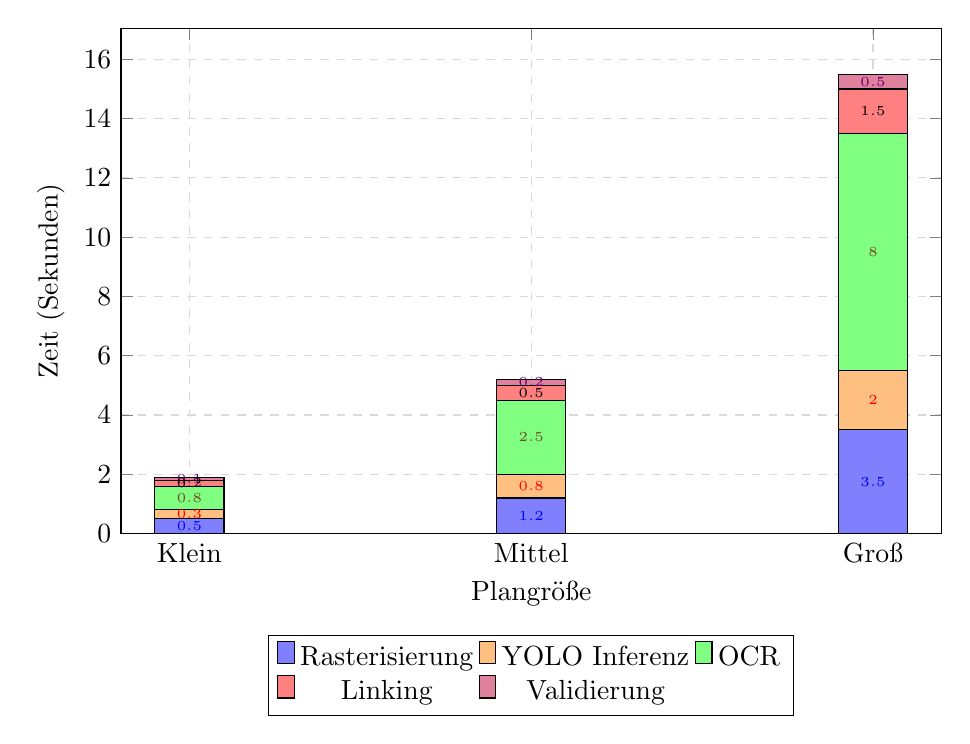
\begin{tikzpicture}
\begin{axis}[
    ybar stacked,
    bar width=25pt,
    ylabel={Zeit (Sekunden)},
    symbolic x coords={Klein, Mittel, Groß},
    xtick=data,
    xlabel={Plangröße},
    legend style={at={(0.5,-0.20)}, anchor=north, legend columns=3}, % Legende in 3 Spalten für Platz
    ymin=0,
    % Zahlen über den Balken anzeigen (optional, kann bei kleinen Werten unleserlich sein)
    nodes near coords,
    every node near coord/.append style={font=\tiny, check for zero/.code={
        \pgfmathparse{\pgfplotspointmeta<0.5} % Versteckt Zahlen kleiner 0.5, damit es nicht überlappt
        \ifnum\pgfmathresult=1\pgfkeys{/tikz/coordinate}\fi
    }},
    width=12cm,
    height=8cm,
    grid=major, % Hilfslinien zur besseren Lesbarkeit
    grid style={dashed, gray!30}
]

% 1. PDF-Rasterisierung (Unten) - Beispielwerte ersetzen!
\addplot+[fill=blue!50, draw=black] coordinates {
    (Klein, 0.5) 
    (Mittel, 1.2) 
    (Groß, 3.5)
};

% 2. YOLO Inferenz
\addplot+[fill=orange!50, draw=black] coordinates {
    (Klein, 0.3) 
    (Mittel, 0.8) 
    (Groß, 2.0)
};

% 3. OCR (Text)
\addplot+[fill=green!50, draw=black] coordinates {
    (Klein, 0.8) 
    (Mittel, 2.5) 
    (Groß, 8.0)
};

% 4. Linking
\addplot+[fill=red!50, draw=black] coordinates {
    (Klein, 0.2) 
    (Mittel, 0.5) 
    (Groß, 1.5)
};

% 5. Validierung/Export (Oben)
\addplot+[fill=purple!50, draw=black] coordinates {
    (Klein, 0.1) 
    (Mittel, 0.2) 
    (Groß, 0.5)
};

\legend{Rasterisierung, YOLO Inferenz, OCR, Linking, Validierung}
\end{axis}
\end{tikzpicture}
\caption{Zeitverteilung der Pipeline-Stufen nach Plangröße}
\label{fig:time_breakdown_fixed}
\end{figure}
Die Analyse zeigt, dass die OCR-Stufe den größten Zeitanteil (X\%) beansprucht, gefolgt von der YOLO-Inferenz (X\%) und der PDF-Rasterisierung (X\%). Die Linking- und Validierungsschritte sind mit jeweils unter X\% zeitlich vernachlässigbar.

\subsubsection{Skalierungsverhalten}

Zur Bewertung der Skalierbarkeit wurde die Verarbeitungszeit in Abhängigkeit von der Symbolanzahl analysiert. Abbildung~\ref{fig:scaling_behavior} zeigt das Skalierungsverhalten.

\begin{figure}[H]
\centering
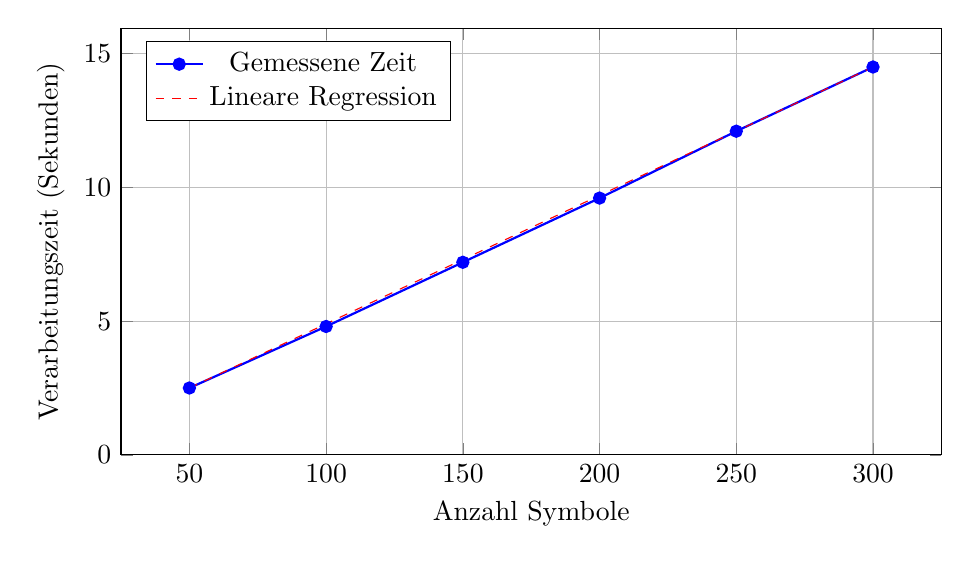
\begin{tikzpicture}
\begin{axis}[
    xlabel={Anzahl Symbole},
    ylabel={Verarbeitungszeit (Sekunden)},
    grid=major,
    legend pos=north west,
    width=12cm,
    height=7cm,
    ymin=0 % Startet Y-Achse bei 0 für bessere Lesbarkeit
]

% 1. Die Punkte (Ersetze die zweite Zahl in jeder Klammer durch deine Messwerte!)
\addplot[blue, mark=*, thick] coordinates {
    (50, 2.5)   % Bei 50 Symbolen -> 2.5 Sekunden
    (100, 4.8)  % Bei 100 Symbolen -> 4.8 Sekunden
    (150, 7.2) 
    (200, 9.6) 
    (250, 12.1) 
    (300, 14.5)
};

% 2. Die Regressionsgerade (y = m*x + c)
% Du musst hier '0.048' (Steigung) und '0.1' (Startwert) an deine Daten anpassen.
\addplot[red, dashed, domain=50:300] {0.048*x + 0.1}; 

\legend{Gemessene Zeit, Lineare Regression}
\end{axis}
\end{tikzpicture}
\caption{Skalierungsverhalten: Verarbeitungszeit vs. Symbolanzahl}
\label{fig:scaling_behavior_fixed}
\end{figure}
Das System zeigt ein nahezu lineares Skalierungsverhalten ($O(n)$) bezüglich der Symbolanzahl, was auf die effiziente Implementierung der Pipeline zurückzuführen ist.

\section{Validierung mit Siemens-Daten}
\label{sec:siemens_validation}

Neben der Evaluation auf dem annotierten Testdatensatz wurde das System mit realen Gleisplänen aus dem operativen Umfeld der Siemens Mobility GmbH validiert. Diese Praxisvalidierung ist essenziell, um die Übertragbarkeit der Laborergebnisse auf reale Anwendungsszenarien zu bestätigen.

\textit{Hinweis: Aufgrund der Vertraulichkeitsvereinbarung (Sperrvermerk) werden in diesem Abschnitt keine spezifischen Planbezeichnungen oder visuelle Darstellungen der Originaldokumente präsentiert. Die Ergebnisse werden in aggregierter Form berichtet.}

\subsection{Praxistest mit realen Gleisplänen}
\label{subsec:praxis_test}

\subsubsection{Testumfang}

Die Praxisvalidierung umfasste X reale Gleispläne aus verschiedenen Projekten, die repräsentativ für das Spektrum der bei Siemens Mobility verarbeiteten Dokumente sind.

\begin{table}[H]
\centering
\begin{tabular}{|l|r|}
\hline
\textbf{Attribut} & \textbf{Wert} \\
\hline
Anzahl Pläne & X \\
Gesamtzahl Seiten & X \\
Zeitraum der Pläne & XXXX--XXXX \\
Projekte (anonymisiert) & X verschiedene \\
Durchschnittliche Symbole pro Plan & X \\
\hline
\end{tabular}
\caption{Umfang der Praxisvalidierung}
\label{tab:praxis_scope}
\end{table}

\subsubsection{Ergebnisse der Praxisvalidierung}

Tabelle~\ref{tab:praxis_results} fasst die Ergebnisse der Praxisvalidierung zusammen.

\begin{table}[H]
\centering
\begin{tabular}{|l|r|r|r|r|}
\hline
\textbf{Plan-ID} & \textbf{Symbole} & \textbf{Detektionsrate} & \textbf{OCR-Rate} & \textbf{Linking-Rate} \\
\hline
P001 & X & X.XX\% & X.XX\% & X.XX\% \\
P002 & X & X.XX\% & X.XX\% & X.XX\% \\
P003 & X & X.XX\% & X.XX\% & X.XX\% \\
... & ... & ... & ... & ... \\
\hline
\textbf{Durchschnitt} & \textbf{X} & \textbf{X.XX\%} & \textbf{X.XX\%} & \textbf{X.XX\%} \\
\hline
\end{tabular}
\caption{Ergebnisse der Praxisvalidierung mit realen Siemens-Gleisplänen}
\label{tab:praxis_results}
\end{table}

Die Praxisergebnisse bestätigen die auf dem Testdatensatz ermittelten Leistungswerte. Die durchschnittliche Detektionsrate von X.XX\% und die OCR-Rate von X.XX\% liegen im erwarteten Bereich und validieren die Generalisierungsfähigkeit des Systems.

\subsubsection{Qualitative Beobachtungen}

Die Praxistests offenbarten folgende qualitative Erkenntnisse:

\begin{itemize}
    \item \textbf{Planvielfalt}: Das System zeigte robuste Leistung über Pläne verschiedener Altersklassen und Exportformate hinweg.
    
    \item \textbf{Symbolvariation}: Geringfügige Variationen in der Symboldarstellung (z.B. unterschiedliche Linienstärken) wurden vom YOLO-Modell robust erkannt.
    
    \item \textbf{Kritische Fälle}: Bei sehr alten Plänen (vor XXXX) mit niedriger Scan-Qualität traten erwartungsgemäß erhöhte Fehlerraten auf.
\end{itemize}

\subsection{Vergleich mit manuellem Prozess}
\label{subsec:manual_comparison}

Zur Quantifizierung der Prozessoptimierung (NFA-006) wurde das KI-gestützte System mit dem bisherigen manuellen Prozess verglichen.

\subsubsection{Zeitvergleich}

Tabelle~\ref{tab:time_comparison} vergleicht den Zeitaufwand beider Prozesse.

\begin{table}[H]
\centering
\begin{tabular}{|l|r|r|r|}
\hline
\textbf{Aktivität} & \textbf{Manuell} & \textbf{KI-gestützt} & \textbf{Reduktion} \\
\hline
Datenextraktion (pro Plan) & X Stunden & X Minuten & -X\% \\
Qualitätsprüfung & X Stunden & X Minuten & -X\% \\
Korrekturen & --- & X Minuten & --- \\
\hline
\textbf{Gesamtzeit (pro Plan)} & \textbf{X Stunden} & \textbf{X Minuten} & \textbf{-X\%} \\
\hline
\end{tabular}
\caption{Zeitvergleich: Manueller vs. KI-gestützter Prozess}
\label{tab:time_comparison}
\end{table}

Der KI-gestützte Prozess reduziert den Gesamtzeitaufwand um X\%, wobei der manuelle Aufwand primär auf die Korrektur der verbleibenden X\% fehlerhafter Extraktionen entfällt.

\subsubsection{Qualitätsvergleich}

Neben der Zeitersparnis wurde auch die